\section{Implementation}
\label{sec:implementation}


\begin{table}
\centering
\begin{tabu} to \textwidth { | l | c |}
    \hline 
    \textbf{Language}      & Line Count \\ \hline
    \textbf{Java}          & 7549       \\ \hline
    \textbf{RenderScript}  & 1000       \\ \hline
    \textbf{JNI/C++}       & 2048       \\ \hline
    \textbf{OpenCL}        & 480        \\ \hline
\end{tabu}
\caption{Lines-of-code project breakdown per language.}
\label{table:breakdown}
\end{table}



Table~\ref{table:breakdown} shows the numbers of lines-of-code (LOC) broken down
into different types of programming languages in the project. This section describe 
how we can achieve good code reuse while still having a sound and understandable program structure.

\subsection{Framework Structure}

\begin{figure}
\centering
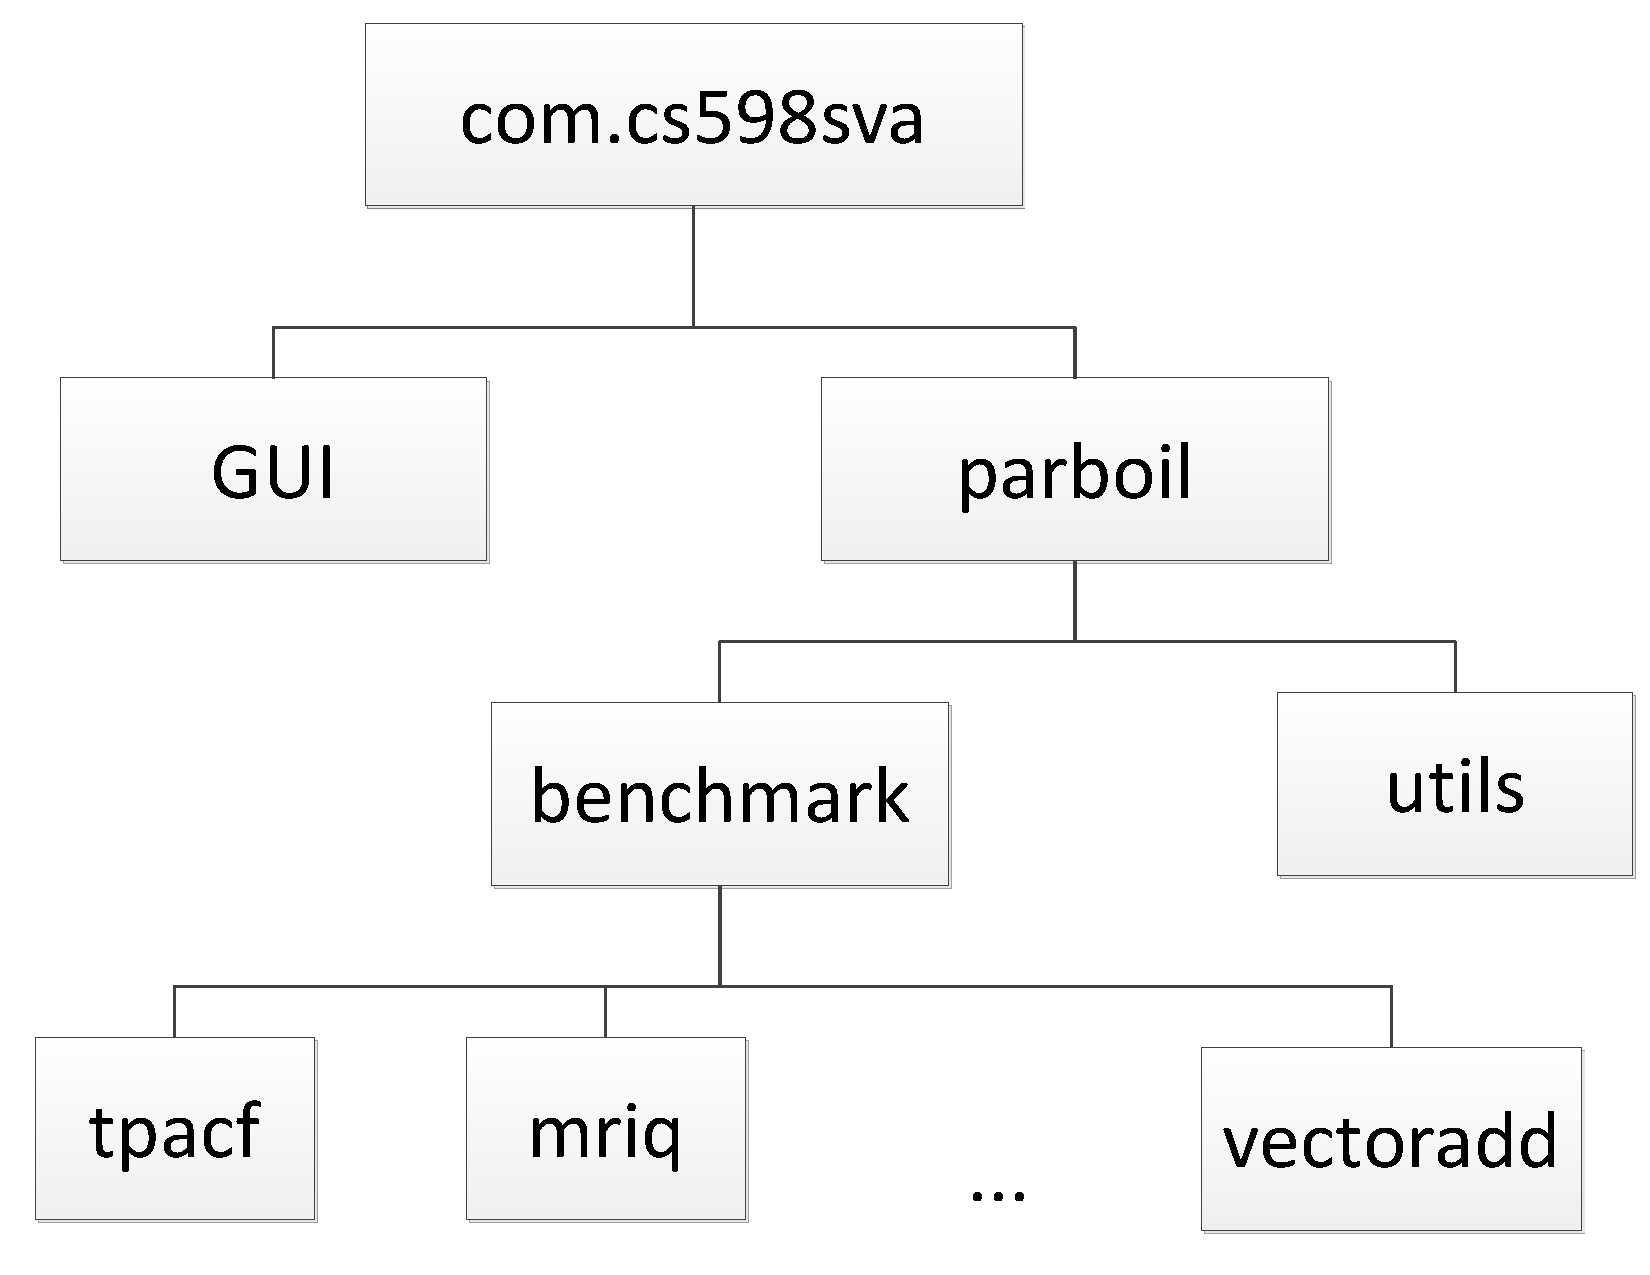
\includegraphics[scale=0.25]{figs/package_diagram.pdf}
\caption{The Java package structure.}
\label{fig:package_structure}
\centering
\end{figure}


\begin{figure}
\centering
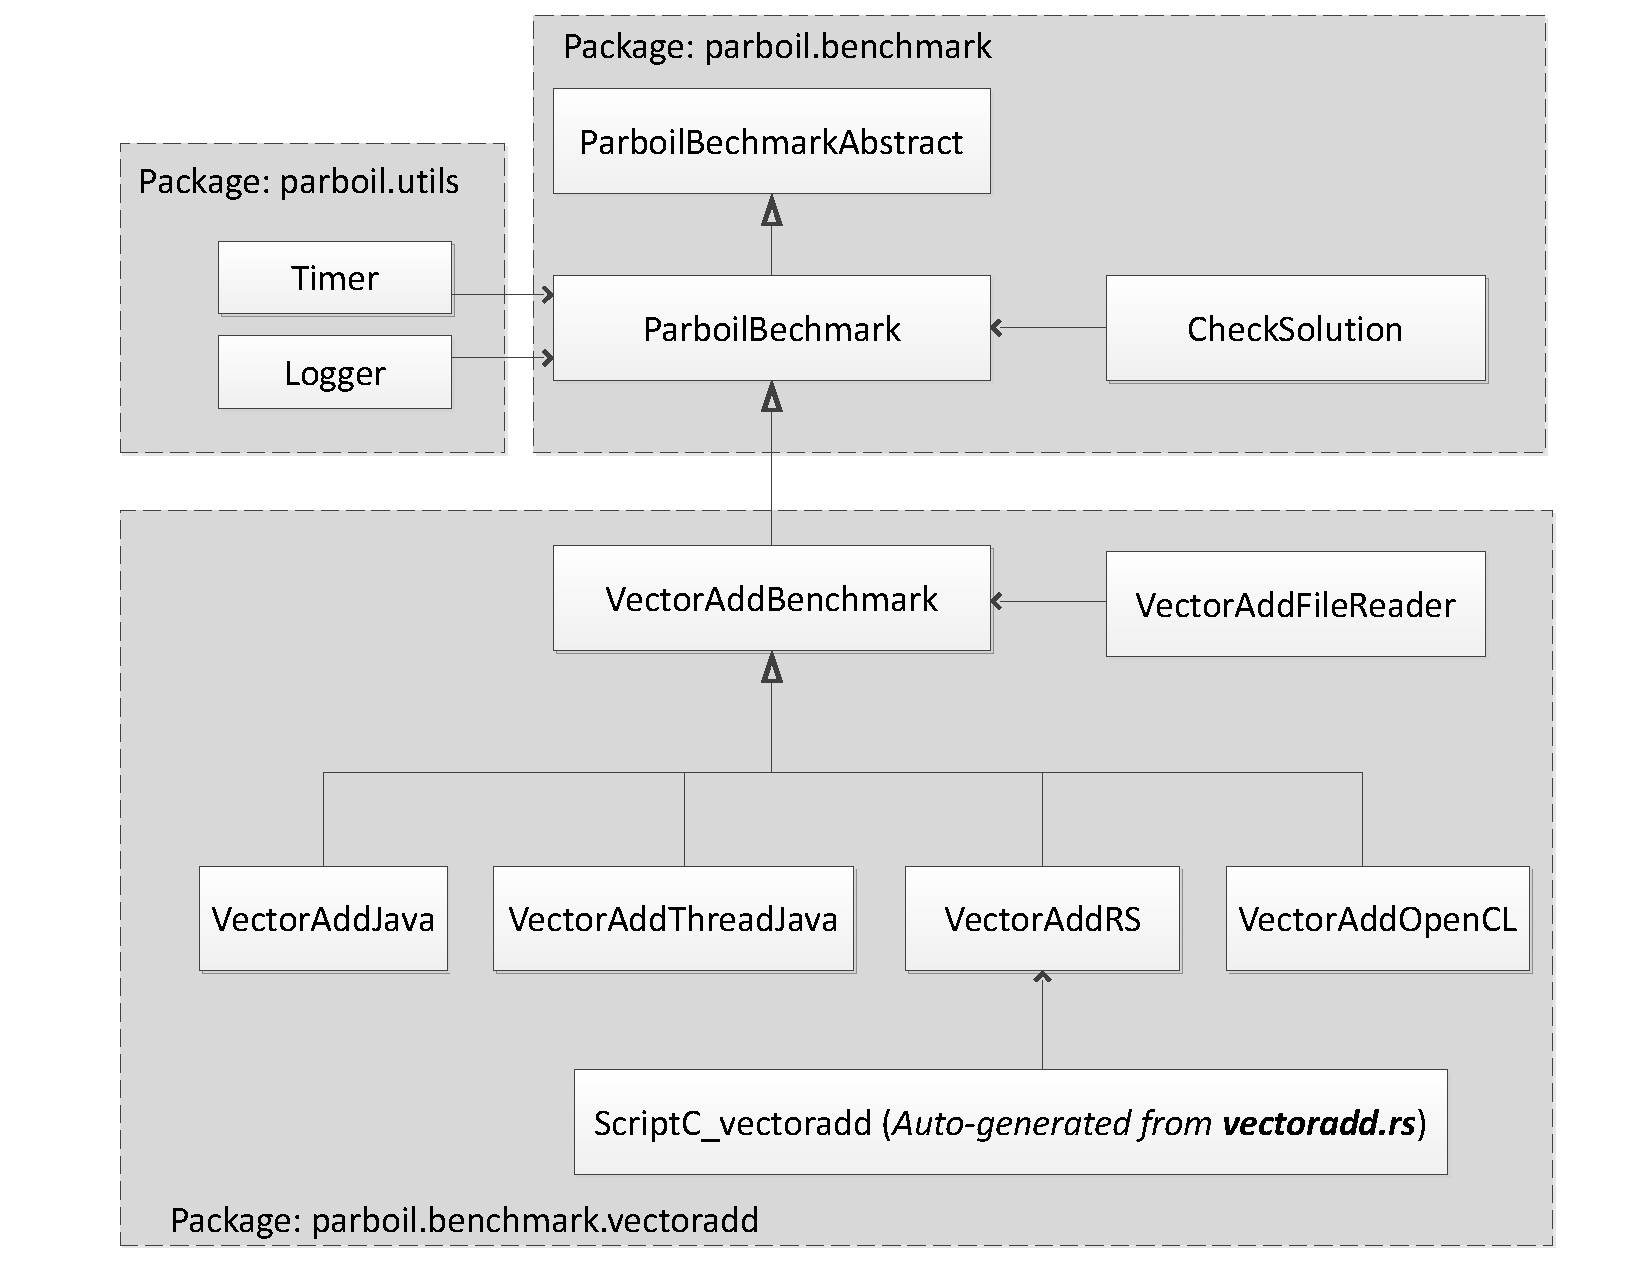
\includegraphics[scale=0.3]{figs/vectoradd_class_diagram.pdf}
\caption{Class diagram of the VectorAdd benchmark.}
\label{fig:class_diagram}
\centering
\end{figure}

We design our framework to serve two purposes.
First, as shown in Figure~\ref{fig:package_structure}, we separated the UI logic from the benchmark logic, furthermore each benchmark is compartmentalized into its own Java package --- this allows for benchmarks to be worked on independently.
Second we make extensive use of subclassing to facilitate code reuse --- 
	we would like to only write one file input handler for each benchmark,
	for example.
Figure~\ref{fig:class_diagram} provides a closer
view at the class hierarchy for the VectorAdd benchmark.

The \fix{parboil} package is the core Java package of the project.
Common utility functions such as timers and loggers are placed in the \fix{utils} package and reused across benchmarks.

Each benchmark's base class has an input and output reader, code to
	initialize the data, and code to check if the output result matches
	the expected output.
The implementation of each benchmark requires one to define just the \fix{compute}
	method.
This design keeps code simple and avoid code duplication.


\subsection{Utility Functions}

A few utility functions were identified to be common across benchmarks.
This section briefly discusses some of them.

\subsubsection{Timer}
The \fix{Timer} class uses \fix{SystemClock} to get real-time clock information 
	with nanosecond resolution.
\fix{Timer} objects are collected into a dynamic list with each measuring
	a particular execution segment, e.g., allocation time, setup time, and compute
time. 
\fix{Timer.start(category, message)} starts the timer and sets its label (here category is a user defined category such as
``Compute'' or ``Setup'', while message is a message that further refines the
category such as ``Allocating temporary data structures''). At the end of the
execution segment the \fix{Time.stop()} method is called. 

Unlike Parboil, which outputs the times to {\tt stdout}, we output our data into
a SQLite database.  This affords us a few things.  First, since data is
outputted in the specified columns, we do not have to re-parse the output data.
Second, timing information can be shared easily by copying the database.
Finally, we can store more than just timing information -- for example we also
store which machine the time has been taken on as well as which runtime is being
used.  Since writing to flash is expensive, all timing data is stored in memory,
and then after the benchmark has finished, it is written into the database. 

\subsubsection{Processor and Power Utilization}

Unlike programming desktops, where one mainly 
  improves software by increasing either features or performance,
  mobile programmers develop for increase features, performance, and 
  battery life.
In fact, one of the main selling points for heterogeneous
  programming on mobile devices, is the increase in battery life.
Increasingly, hardware vendors, such as Apple or Samsung, sell new
  mobile hardware by advertising longer battery life.
Finding a balance between energy consumption and performance is a 
  balancing act that a programmer would like to delegate to the 
  compiler or runtime.

Since Android does not offer a way to capture processor usage information
programmatically, we use the Trepn~\cite{profilerqualcomm} tool by Qualcomm to capture the data and save it into a {\tt csv} file.
This tool is limited to Qualcomm based
chipsets. Trepn reads internal processor counters as well as power rail information,
both of which are not available programmatically and are more accurate than reading
the information from the \fix{/proc} kernel file system.

Trepn is an external application that is run outside of our benchmark framework.
To pass messages to Trepn, we make use of Android's \fix{Intent} framework.
The \fix{Intent} framework allows one to pass messages between applications.
Trepn records the time a message is received (which corresponds to time blocks
in our code) and we developed scripts to correlate Trepn's data dump with both
the load and power usage.

We set Trepn to read
the counters every $100ms$ and measure the load and power usage separately to
decrease the overhead of the profiler.  To reduce overhead, Trepn measures the
processor usage information every $100ms$, both the frequency and the load are
measured sequentially, we therefore needed to correct that when parsing the {\tt
csv} file.

First, we parse each processor reading along with the time-stamps for reading the
file.  Next, we interpolate the measured data (we use linear interpolation), and
evaluate the interpolated value at the application state times (these are the times
Trepn received signals from our application and correspond to timed blocks of
code).  We then multiply the load by the frequency, and rescale all the CPU and
GPU data (we perform the rescaling on the CPU and GPU separately).  Trepn can
have measurement errors, resulting in infinite numbers.  To make sure that these
do not skew the plots, we clip the range of possible processor reading to be
between 1 and $0.99$th quantile of the data.  While efforts have
been taken to reduce the profiler's overhead, the overhead is still around
$10\%$.

\subsection{Compute Kernels}

A RenderScript kernel is a map operation, taking a sequence of input and producing one output. For example, in
the VectorAdd benchmark, the kernel takes two elements (one from each vector) adds the results and produces an output.
With sequential accesses, one does not need to index into an array to access elements. In general, this results in code that's simpler to understand than OpenCL. 

RenderScript does not unify memory, but provides APIs from within Java to allocate data and copy to and from the runtime. 
We use \fix{copyFromUnchecked} to perform unsafe copies between Java and RenderScript, otherwise the runtime allocate temporary buffers and checks whether the conversion between the Java type and RenderScript type is valid.

The RenderScript targets the $4.4$ Android platforms and 
	is compiled with \fix{renderscript.support.mode=false} which
	allows the compiler to use some optimizations which were not available in
	previous Android versions.

Since Android applications must be hosted within Dalvik VM, we write JNI to 
	interface our code with the native 
	--- C, OpenMP, and OpenCL. To avoid having to write another timer, 
	we split the native code into JNI functions corresponding to timed blocks and our
	Java timer is used to time the native code.
	Aside from
wrapping the code via JNI so it is callable from within Java, little
modification was done to the Parboil version of the C and OpenMP code.


The OpenCL kernels are lifted from Parboil as well, but we rewrite the 
	OpenCL host code using the C++ OpenCL API, since it simplifies some of the
	code and affords more code reuse opportunities.
We use the \fix{base} implementation of OpenCL --- this a
platform agnostic unoptimized implementation.

To allow devices with no OpenCL support to make use of the C and OpenMP
implementations, we generate 3 libraries (one for C, OpenMP, and OpenCL).  Each
library is then loaded and called from with its class implementation.
The \fix{-O3 -ftree-vectorize -mvectorize-with-neon-quad}
 compile option  is set when compiling the libraries, this allows the compiler the opportunity to autovectorization code.
